
\chapter{Flavour Tagging with Graph Networks and Transformers}
\label{ch:spice}

In this chapter we describe the design and implementation new graph networks for flavour tagging.
Jet flavour tagging is a crucial part of the ATLAS experiment and is described in \Cref{sec:flavour_tagging}.
These models attempt to identify the flavour of a jet based on the properties of the reconstructed charged particle tracks associated with it.

The new models build on GN1, a graph network which uses GATv2 system of message passing~\cite{GATv2}.
The first new model is called GN++ and is based on the full GN-Block architecture described in \Cref{sec:gn_block}, complete with persistent edge information and global attributes.
The second new model is called Spice and is based on the transformer-encoder architecture, described in \Cref{sec:transformer}.
Spice would prove to be so performant and efficient that it would form the basis of the new GN2 flavour tagger adopted by the ATLAS collaboration.

One of the observations made over the course of this project is that the rate of progress in machine learning is much faster than in high energy physics.
At the time Spice was being developed and presented to the flavour tagging group, GN1 was still undergoing collaboration.
At the time of writing, GN2 is now being calibrated, and significant effort is being used to keep it up to date with the latest developments in machine learning.
One of the main contributions of this thesis was the development of Salt~\cite{Salt}, a repository for training transformers for flavour tagging which is constantly being updated with the latest models and training techniques.

\section{Datasets}

Training and evaluating GN++ and Spice required the use of simulated datasets in order to provide a ground truth for the jet flavour.
This work reuses the same samples as the previous flavour taggers, DIPS and GN1, and further information can be found in \textcite{AlexThesis} and Ref.~\cite{GN1}.
The training datasets are selected to cover a wide range of $\pt$ values and further resampled to ensure that the jet $\pt$ and $\eta$ distributions are identical for the three jet flavours used in the classification, namely $b$-, $c$-, and light-jets.

Two simulated datasets are used.
The first dataset comprises $\ttbar$ events, primarily covering the $\pt < 250~\GeV$ phase space.
The simulation settings for this sample were derived from best fits of the data distributions for jet multiplicity and top quark momentum~\cite{ttbar1, ttbar2}.
The second dataset consists of $Z'$ events, included to enhance the training statistics in the high $\pt$ phase space.
The $Z'$ boson, a non-SM particle, is designed explicitly with cross-section of the hard scattering process adjusted to produce a flat mass distribution, leading to a relatively uniform distribution of jets with $\pt$ up to $5~\TeV$.
The branching fractions were also tuned to result in a roughly equal distribution of $b$-, $c$-, and light-jets at $\pt \approx 3~\TeV$.
The branching fractions of the $Z'$ boson shown in \Cref{tab:zprime_branching}.

Distributions of the jet $\pt$ and $\eta$ for the two datasets are shown in \Cref{fig:jet_pt_eta}.

\begin{table}[h]
    \centering
    \begin{tabular}{lcc}
        \toprule
        \midrule
        Decay Mode & Branching Fraction \\
        \midrule
        $b\bar{b}$ & 0.30 \\
        $c\bar{c}$ & 0.30 \\
        $s\bar{s}$ & 0.10 \\
        $d\bar{d}$ & 0.10 \\
        $u\bar{u}$ & 0.10 \\
        $\tau^-\tau^+$ & 0.05 \\
        $e^-e^+$ & 0.05 \\
        \bottomrule
    \end{tabular}
    \caption{Branching fractions for the $Z'$ boson \cite{Run2FTAlgs}}
    \label{tab:zprime_branching}
\end{table}


\begin{figure}
    \centering
    \begin{subfigure}[b]{0.49\textwidth}
        \centering
        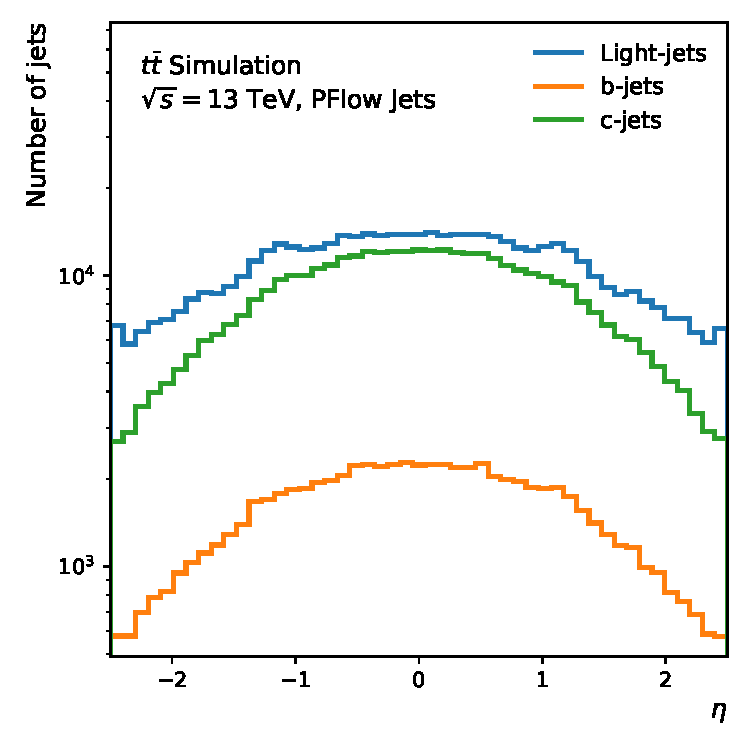
\includegraphics[width=\textwidth]{figures/flavour_tagging/ttbar_0.pdf}
        \caption{$\ttbar$ jet $\eta$ distribution}
        \label{fig:ttbar_eta}
    \end{subfigure}
    \begin{subfigure}[b]{0.49\textwidth}
        \centering
        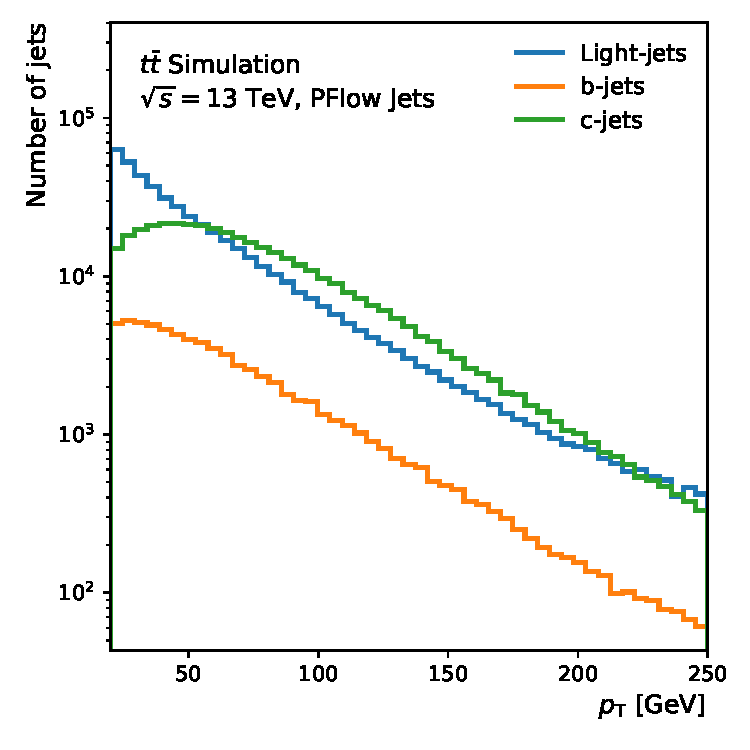
\includegraphics[width=\textwidth]{figures/flavour_tagging/ttbar_1.pdf}
        \caption{$\ttbar$ jet $\pt$ distribution}
        \label{fig:ttbar_pt}
    \end{subfigure}
    \begin{subfigure}[b]{0.49\textwidth}
        \centering
        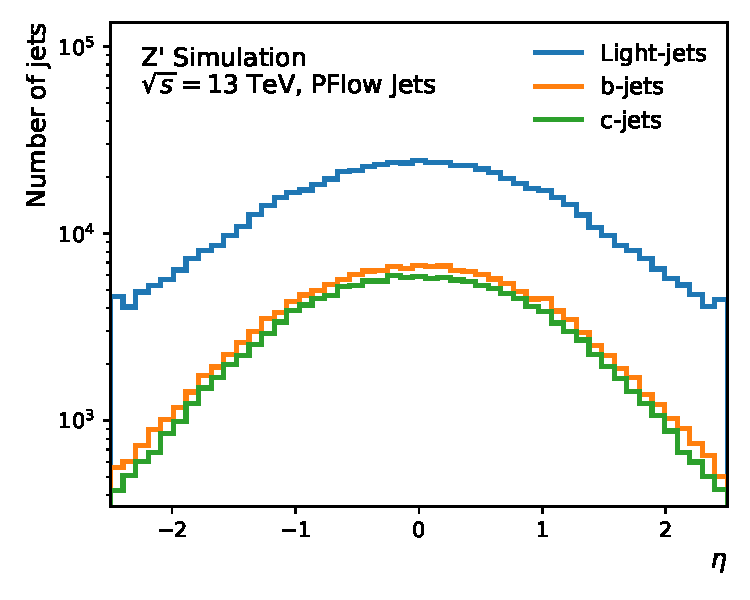
\includegraphics[width=\textwidth]{figures/flavour_tagging/zprime_0.pdf}
        \caption{$Z'$ jet $\eta$ distribution}
        \label{fig:zprime_eta}
    \end{subfigure}
    \begin{subfigure}[b]{0.49\textwidth}
        \centering
        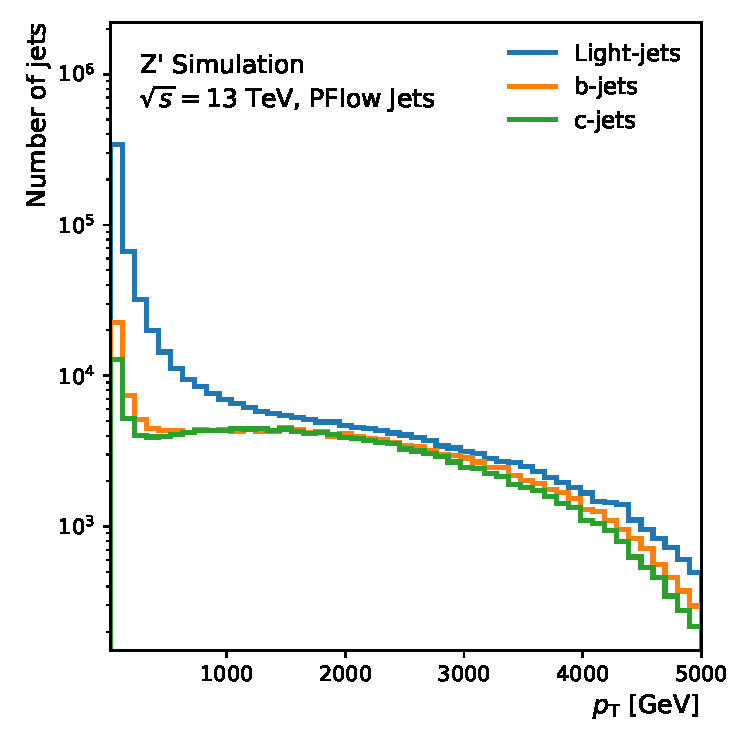
\includegraphics[width=\textwidth]{figures/flavour_tagging/zprime_1.pdf}
        \caption{$Z'$ jet $\pt$ distribution}
        \label{fig:zprime_pt}
    \end{subfigure}
    \caption{Original (non-resampled) jet $\pt$ and $\eta$ distributions for the $\ttbar$ and $Z'$ datasets.}
    \label{fig:jet_pt_eta}
\end{figure}

\subsection{Monte Carlo Generation}

Both datasets are initiated by simulated proton-proton collisions at a center-of-mass energy of $\sqrt{s} = 13$ TeV.

Hard scatter events for the $\ttbar$ sample were generated at next-to-leading order using \textsc{PowhegBox v2}~\cite{Powheg1, Powheg2, Powheg3}.
These events then interfaced with \textsc{Pythia 8.230}~\cite{Pythia8} using the \textsc{A14} tune~\cite{A14} for parton showering and hadronization.
For the parton distribution functions, the \textsc{NNPDF3.0NNLO}~\cite{PDF3.0} set was used for the matrix element calculation while the \textsc{NNPDF2.3LO}~\cite{PDF2.3} set was used for the showering.
The cut-off scale parameter for the first-gluon-emission $h_{\text{damp}}$ was set to 1.5 times the top quark mass of $m_t = 172.5~\GeV$.
The $Z'$ sample was generated and showered using \textsc{Pythia 8.212} with the \textsc{A14} tune and the \textsc{NNPDF2.3LO} set of parton distribution functions.
The flat mass distribution of the $Z'$ boson was achieved by applying a per-event weight to broaden the natural decay width of the $Z'$ boson.

For both datasets, decays of $b$- and $c$-hadrons were simulated using the \textsc{EvtGen v1.6.0} package \cite{EvtGen}.
Detector response was performed using the \textsc{Geant4} simulation package~\cite{Geant4} with the ATLAS simulation setup~\cite{ATLASSim}.
These signals are combined with the hard scatter events during the digitization step.
Interactions with heavy flavour hadrons and the detector material was not simulated but accounted for in correction factors and systematic uncertainties.
Pileup was modelled by overlaying extra minimum bias events using the \textsc{Pythia 8.160} generator with the \textsc{A3} tune~\cite{A3} and the \textsc{NNPDF2.3LO} parton distribution functions.
In-time pileup was modelled using an average of 40 interactions per bunch crossing, while out-of-time pileup was modelled using bunch crossings before and after the primary interaction.

\subsection{Reconstruction}

The output of the simulation was reconstructed using the standard ATLAS reconstruction procedure described in \Cref{sec:event_reconstruction}.
In these experiments, the inputs to the model stem from the tracks and no calibrated physics objects, such as reconstructed photon, electrons, or muons, are used.

Charged particle tracks are required to pass the loose selection criteria~\cite{TrackLoose} as shown in \Cref{tab:track_loose}.
The hard scatter primary vertex (PV) is defined as the vertex with the highest sum of squared transverse momenta of the associated tracks.
The impact parameters (IPs) for each track are measured with respect to the PV of the event.
Jets are reconstructed from particle-flow objects~\cite{PFlow} using the anti-$k_t$ algorithm with a radius parameter of $R = 0.4$.
More details are covered in \Cref{sec:particle_flow}.
Tracks are associated to a jet based on the $\Delta R$ separation to the jet axis.
The threshold decreases as a function of the jet $\pt$ to account for the increased collimation of the jet cone, from $\Delta R = 0.45$ at $\pt = 20~\GeV$ to $\Delta R = 0.25$ at $\pt \geq 200~\GeV$.
If a track associated with multiple jets, it is assigned to the jet with the smallest $\Delta R$ separation.

\begin{table}
    \centering
    \begin{tabular}{ll}
        \toprule
        \midrule
        \multicolumn{2}{c}{Track Loose Selection Criteria} \\
        \midrule
        $\pt$ & $> 1~\GeV$ \\
        $d_0$ & $< 3.5~\mm$ \\
        $z_0 \sin \theta$ & $< 5~\mm$ \\
        Number of hits in the SCT & $\geq 8$ \\
        Number of hits shared by other tracks & $\leq 2$ \\
        Number of SCT holes & $\leq 3$ \\
        Number of pixel holes & $\leq 2$ \\
        \bottomrule
    \end{tabular}
    \caption{Loose selection criteria for charged particle tracks~\cite{TrackLoose}.}
    \label{tab:track_loose}
\end{table}

\subsection{Truth Labelling}

As with GN1, these networks are trained to perform three complimentary tasks.
There is task is the classification of the jet flavour, this is the primary task.
The second task is to predict the origin of each track within the jet.
The final task is to segment the jet: given any two tracks from the same jet, determine if they emerged from the same vertex.
Each of these requires defining ground truth labels.

The truth labelling of the jets is based on the existence of generator level particles within a $\Delta R$ separation of 0.3.
The jet is associated with the particle with the highest priority within this radius.
The considered particles in order of decreasing priority are, $b$-hadrons, $c$-hadrons, and $\tau$ leptons, which will result in the jet being labelled as a $b$-jet, $c$-jet, $\tau$-jet respectively.
If no such particles are found, the jet is labelled as a light-jet.
We discard $\tau$-jets for this study.

The truth track origins describe the physical process which produced the track.
First a track is associated with a truth particle by matching its reconstructed hits to the simulated hits of the particle made during the \textsc{Geant4} simulation.
This matching criteria is performed using the~\textit{truth-matching probability} (TMP)~\cite{TMP}.
The TMP constructs a ratio of the matched hits to the total number of hits in the track, with added factors to account for the varying hit efficiencies of the detector subcomponents, namely the pixel, SCT, and TRT detectors.
Each track is associated to the truth particle with the highest TMP.
If no truth particle leads to a TMP greater than 0.75, the track is labelled as a fake track, and it is determined to have originated from multiple overlapping particles.
There are seven possible truth labels for the tracks as shown in \Cref{tab:track_labels}.

\begin{table}
    \centering
    \begin{tabular}{ll}
        \toprule
        \midrule
        Origin & Description \\
        \midrule
        fromB & $b$-hadron decay \\
        fromBC & $c$-hadron decay, which itself originated from a $b$-hadron \\
        fromC & other $c$-hadron decays \\
        OtherSecondary & other secondary decays (such as kaons) \\
        Pileup & a pileup $pp$ interaction \\
        Primary & the primary vertex and not a secondary decay \\
        Fake & multiple overlapping particles \\
        \bottomrule
    \end{tabular}
    \caption{The seven possible truth labels for the tracks.}
    \label{tab:track_labels}
\end{table}

Finally, the truth vertex labelling is based on the origin of the tracks.
This is a simple binary label which determines if a pair of tracks emerged from the same secondary vertex within the jet.
The label is set to True if the associated truth particles of each track share an origin within $1~\mm$ of each other.
If one of the tracks is labelled as Fake or Pileup, the pair is always labelled as False.

\subsection{Selection and Sampling}

Jets are required to have $\pt > 20~\GeV$ and $|\eta| < 2.5$ and may not overlap with a generator-level lepton from a $W$ or $Z$ decay.
From the $Z'$ sample, jets are further required to have $\pt > 250~\GeV$ to avoid simulation artefacts.
All jets with $\pt < 60~\GeV$ and $|\eta| < 2.4$ must also pass the tight working point of the JVT algorithm in order to minimize contributions from pileup~\cite{JVT}.

As shown in \Cref{fig:jet_pt_eta}, there is a significant difference between the jet $\pt$ and $\eta$ for the three jet flavours.
This would bias the training of the model and lead to issues down the line for calibration.
To mitigate this, the training dataset is resampled with replacement to ensure that the 2D distribution of jet $\pt$ and $\eta$ is identical for the three jet flavours~\cite{AlexThesis}.

After resampling the training set contained a total of 120 million jets split equally between the three jet flavours and composed of a mixture of around 70\% $\ttbar$ and 30\% $Z'$ events.
The distributions of the jet $\pt$ and $\eta$ for the resampled datasets are shown in \Cref{fig:train_jet_pt_eta}.
During training, 5\% of this was reserved for hold out validation.

Two statistically independent test samples were produced, each containing 1 million $\ttbar$ and $Z'$ jets respectively.
No resampling was performed on the test datasets.

\begin{figure}
    \centering
    \begin{subfigure}[b]{0.49\textwidth}
        \centering
        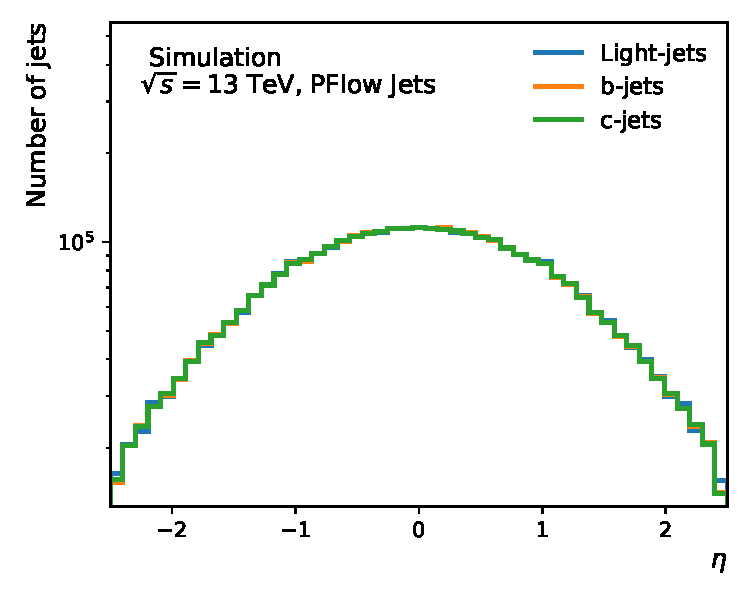
\includegraphics[width=\textwidth]{figures/flavour_tagging/train_0.pdf}
        \caption{Training set $\eta$ distribution}
        \label{fig:train_eta}
    \end{subfigure}
    \begin{subfigure}[b]{0.49\textwidth}
        \centering
        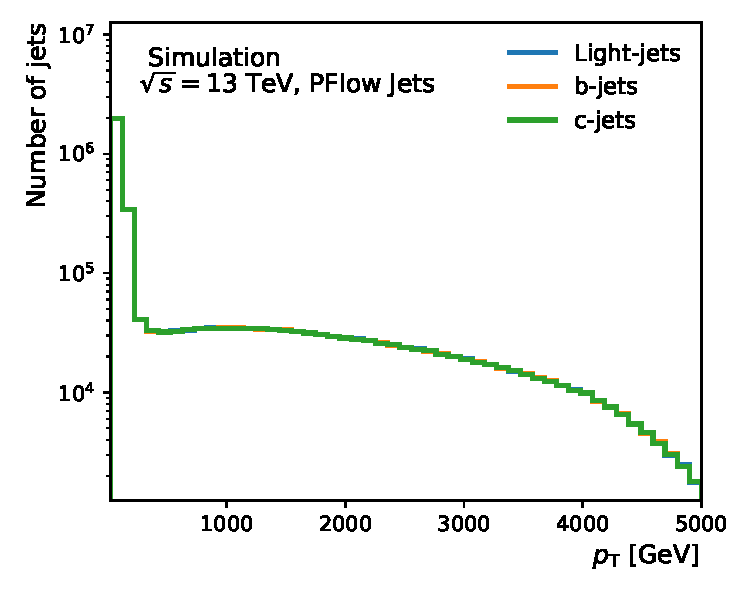
\includegraphics[width=\textwidth]{figures/flavour_tagging/train_1.pdf}
        \caption{Training set $\pt$ distribution}
        \label{fig:train_pt}
    \end{subfigure}
    \caption{Resampled jet $\pt$ and $\eta$ distributions for the $\ttbar$ training dataset. For these plot only 10M jets were selected as a representative sample.}
    \label{fig:train_jet_pt_eta}
\end{figure}

\subsection{Input Features}

The inputs to all models are the same as those used in GN1.
They include two kinematic jet variables, $\pt$ and $\eta$, and up to 40 tracks associated with the jet.
Each track is represented by a vector containing 21 features, detailed in \Cref{tab:track_features}.
Almost all $\ttbar$ jets contain less than 40 tracks, but a significant fraction of $Z'$ jets contain more, as shown in \Cref{fig:track_multiplicity}.
For these samples only the 40 tracks with the highest transverse IP significance $s(d_0)$ are retained.
All features are standardized to have zero mean and unit variance using the training set statistics.
Distributions of the first 5 track features are shown in \Cref{fig:track_features}.

\begin{figure}
    \centering
    \begin{subfigure}[b]{0.49\textwidth}
        \centering
        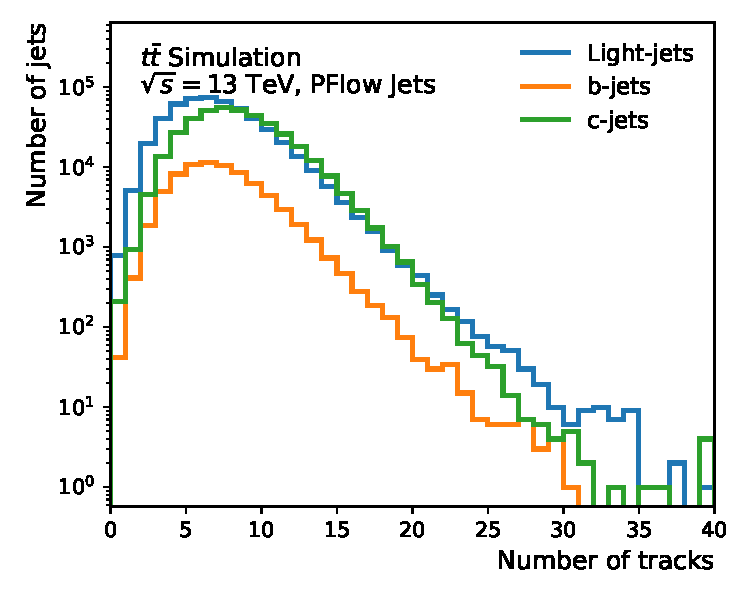
\includegraphics[width=\textwidth]{figures/flavour_tagging/ttbar_2.pdf}
        \caption{Number of tracks per $\ttbar$ jet}
        \label{fig:train_eta}
    \end{subfigure}
    \begin{subfigure}[b]{0.49\textwidth}
        \centering
        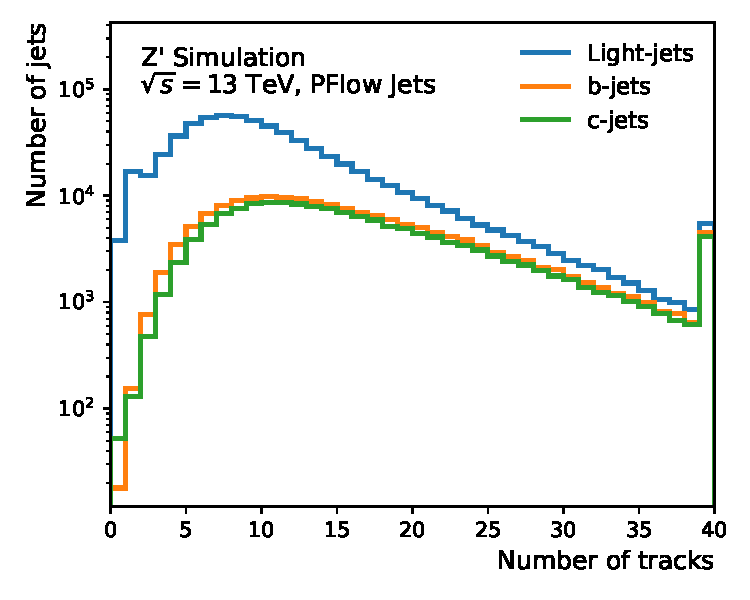
\includegraphics[width=\textwidth]{figures/flavour_tagging/zprime_2.pdf}
        \caption{Number of tracks per $Z'$ jet}
        \label{fig:train_pt}
    \end{subfigure}
    \caption{Original (non-resampled) number of tracks associated with each jet.}
    \label{fig:track_multiplicity}
\end{figure}

\begin{table}[h]
    \centering
    \begin{tabular}{ll}
        \toprule
        \midrule
        \multicolumn{2}{c}{Jet Level Inputs} \\
        \midrule
        $\pt$ & Jet transverse momentum \\
        $\eta$ & Signed jet pseudorapidity \\
        \midrule
        \midrule
        \multicolumn{2}{c}{Track Level Inputs} \\
        \midrule
        $q/p$ & Track charge divided by momentum \\
        $\Delta\eta$ & Pseudorapidity of the track relative to the jet $\eta$ \\
        $\Delta\phi$ & Azimuthal angle of the track relative to the jet $\phi$ \\
        $d_0$ & Closest distance from the track to the PV in the longitudinal plane \\
        $z_0 \sin \theta$ & Closest distance from the track to the PV in the transverse plane \\
        $\sigma(q/p)$ & Uncertainty on q/p \\
        $\sigma(\theta)$ & Uncertainty on track polar angle $\theta$ \\
        $\sigma(\phi)$ & Uncertainty on track azimuthal angle $\phi$ \\
        $s(d_0)$ & Lifetime signed transverse IP significance \\
        $s(z_0)$ & Lifetime signed longitudinal IP significance \\
        nPixHits & Number of pixel hits \\
        nSCTHits & Number of SCT hits \\
        nIBLHits & Number of IBL hits \\
        nBLHits & Number of B-layer hits \\
        nIBLShared & Number of shared IBL hits \\
        nIBLSplit & Number of split IBL hits \\
        nPixShared & Number of shared pixel hits \\
        nPixSplit & Number of split pixel hits \\
        nSCTShared & Number of shared SCT hits \\
        nPixHoles & Number of pixel holes \\
        nSCTHoles & Number of SCT holes \\
        \bottomrule
    \end{tabular}
    \caption{Input features for the graph network flavour taggers.}
    \label{tab:track_features}
\end{table}

\section{Model Design}

All the proposed models can be thought of as variations or extensions of GN1.
Both Spice and GN++ follow this same setup but with updates to the message passing steps as well as latest trends in architecture design.
From~\textcite{RelationalInductiveBiases} comes the design of the GN-Block which include features such as, persistent edge information, persistent global information, and node feed-forward layers.
In addition, we experimented with the transformer architecture along with, PreNorm, conditioning, and residual additive connections which were back fitted to the GN-Block.

GN1 introduced the idea of a monolithic graph neural network which would simultaneously perform jet tagging, track identification, and vertexing.
The input data is a set attributed nodes (the tracks) with an associate global attribute (the jet kinematics), with no explicit graph structure or edges features.
The three training objectives are equivalent to performing a graph level tasks, a node level task, and an edge level task respectively.
Thus, one can think of these models as mappings from the graph structure $(\mathcal{N}, \emptyset, \u) \rightarrow (\mathcal{N}', \mathcal{E}', \u')$, and the loss is calculated on each of the three outputs.

For all the models, while the edges are featureless, they are designed to be fully-connected, meaning that each node sends a message to every other node in the graph.
This was found to improve performance of all models, and the computational overhead was not significant, as the number of tracks per jet was limited to 40.
To compare these models we use flowcharts of the operations within the layers.
Theses flowcharts are shown in \Cref{fig:gn1_graph}, \Cref{fig:gnpp_graph}, \Cref{fig:gnmm_graph}, and \Cref{fig:spice_graph} and use the key shown in \Cref{fig:key}.

\begin{figure}
    \centering
    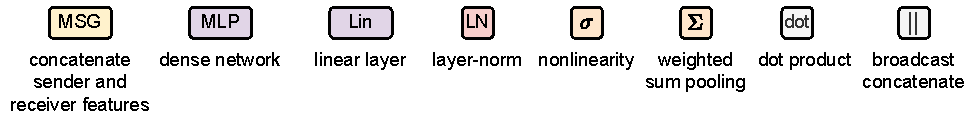
\includegraphics[width=0.99\textwidth]{figures/flavour_tagging/key.pdf}
    \caption{Key for the flowcharts of the graph network operations.}
    \label{fig:key}
\end{figure}

\subsection{GN1}

To better highlight the changes made in GN++ and Spice, we first describe the specifics of the GN1 model.
It is worth highlighting that we are comparing to the original GN1 model as described in Ref.~\cite{GN1}, as later variants began to adopt more transformer like features, such as multi-headed attention and multiple projection matrices before the full shift to Spice/GN2.

The model begins with a track initializer, which is an MLP that takes as inputs the concatenated track and jet features and outputs a track embedding of size 64.
The embedded track features are then passed through a three GATv2 layers~\cite{GATv2} to produce a set of updated track features.
In each layer the track features are projected using a learnable square matrix $\W$.
This is used to simultaneously calculate the message sent between each pair of tracks as well as the message weight using,
\begin{equation}
    e_{ij} = \text{softmax}_i\left(\ba \cdot \relu\left([\W \x_i, \W \x_j]\right)\right),
\end{equation}
where $\ba$ is a learnable vector, and $e_{ij}$ is the message weight sent from node $i$ to node $j$.
The softmax function is applied to all incoming messages to node $j$ to ensure that the weights sum to one.
The messages are then aggregated to update the node information across the graph,
\begin{equation}
    \x_j' = \relu\left(\sum_{i} e_{ij} \cdot \W \x_j\right).
\end{equation}
GN1 uses three of these layers to build its main feature extractor, returning a set of updated node features.
To perform the graph level task, the node features are aggregated using a weighted sum to create a pooled graph representation.
The weights of this sum are derived from another learnable projection on the final node features.
The pooled representation is passed through an MLP called the graph network to produce an output vector of size 3, which can be used for the classification task.
For the node task, the output of the last GATv2 layer is concatenated with the pooled graph representation and passed through another MLP called the node network with 7 outputs.
Finally, for the edge task, node features are concatenated in pairs, with both orderings, together with the pooled features and passed through a third MLP called the edge network 1 output.
In total GN1 has 820k trainable parameters.

There are a number of potential improvements to be made with this design that can be seen as enhancing the graph network structure of the model.
A schematic diagram of the operations taking place within the GN1 graph network is shown in \Cref{fig:gn1_graph}.
To start, the GATv2 layers reuse the same projection matrix $\W$ for both the message calculation and the message weight calculation.
These operations could be performed better with dedicated layers.
Most notably missing is any strong nodewise updates after the message passing.
Framing this in the context of the GN-Block means that the node update $\phi^v$ is simply a ReLU activation function.
The addition of normalization layers, residual connections, and an extension to multi-headed attention could also improve performance.
Other elements such as persistent global or edge information could also be added to the model.

\begin{figure}
    \centering
    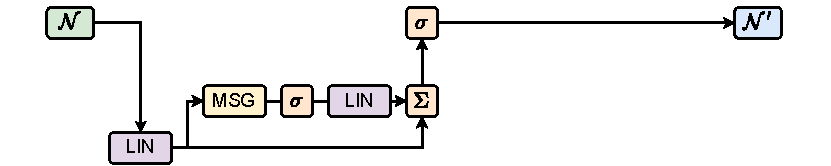
\includegraphics[width=0.99\textwidth]{figures/flavour_tagging/gn1.pdf}
    \caption{Schematic diagram of the operations within the GN1 tagger.}
    \label{fig:gn1_graph}
\end{figure}

\subsection{GN++}

The GN++ model is based on the full GN-Block architecture described in \Cref{sec:gn_block}.
This model is designed to be a more complete graph network, with persistent edge information and global attributes.
The focus of this model is to improve the expressivity of GN1 and thus the performance of the tagger.

A diagram of the information flow within the GN++ model is shown in \Cref{fig:gnpp_graph}.
In a single layer, there are 5 MLPs, 3 to perform the updates $\phi^x$, $\phi^e$, and $\phi^u$, and two to calculate the attention weights for the $\rho^{e \to x}$ and $\rho^{x \to u}$ steps.
The only part omitted from the GN-Block is the $\rho^{e \to u}$ pooling operation as we found that it was computationally expensive and did not improve performance.
Each of the updates for the edges, nodes, and global attributes follows the same pattern, shown in the algorithm in \Cref{alg:gnpp} and by the diagram in \Cref{fig:gnpp_graph}.


\begin{algorithm}
    \caption{The full GN++ block. All MLPs have a LayerNorm operation applied to their inputs and all weight calculations are followed by a softmax operation.}
    \label{alg:gn_block}
    \begin{algorithmic}[1]
        \State \textbf{Input:} Graph attributes $\mathcal{G} = (\mathcal{N}, \mathcal{E}, \u)$
        \State \textbf{Output:} Updated graph attributes $\mathcal{G}' = (\mathcal{N}', \mathcal{E}', \u')$
        \For{each edge $\edge_k$ in $\mathcal{E}$}
            \State $\edge_k' \gets \text{MLP}_e([\edge_k, \x_{s_k}, \x_{r_k}, \u]) + \edge_k$ \Comment{residual update edge features}
            \State $\w_k \gets \text{MLP}_{e \to x}([\edge_k, \x_{s_k}, \x_{r_k}, \u])$ \Comment{calculate edge weights}
        \EndFor
        \For{each node $\x_i$ in $\mathcal{N}$}
            \State $\mathbf{\bar\edge}_i \gets \sum_{k: r_k = i} \w_k \edge_k'$ \Comment{attention pool edges}
            \State $\x_i' \gets \text{MLP}_v([\mathbf{\bar\edge}_i, \x_i, \u])$ \Comment{update node features}
            \State $\w_i \gets \text{MLP}_{x \to u}([\mathbf{\bar\edge}_i, \x_i, \u])$ \Comment{calculate node weights}
        \EndFor
        \State $\mathbf{\bar{x}} \gets \sum_{i} \w_i \x_i'$ \Comment{attention pool nodes}
        \State $\u' \gets \text{MLP}_u([\mathbf{\bar{x}}, \u])$ \Comment{update global attributes}
    \end{algorithmic}
\end{algorithm}


For this model we keep the track initializer from GN1.
However, the three networks for the graph, node, and edge tasks are no longer required as the GN-Block already has expressions for the node and edge tasks.




% - Describe the 3 tier loss
% - Describe the full GNN model
% - Describe the proposed transformer model

\section{Training}

% - Training highlights
% - Loss curves
% - All training parameters

\section{Performance}

% - Output distributions
% - ROC curves
% - Rejection values

\section{Applications}

% - Salt
% - GN2X
% - Current model architecture
% - Current training set
% - Current performance






